\section{Resultados}
    \subsection{Distribución de frecuencias del consumo}
        Con $n = 120$, la regla de Sturges arroja $k = 8$ clases de amplitud 457,0 kWh
        sobre el recorrido comprendido entre 121,2 y 3.777,1 kWh. Antes de leer las
        frecuencias conviene saber quién ocupa cada clase, pues los tres sectores cubren
        franjas de consumo que apenas se solapan y, en consecuencia, cada clase resulta
        casi de un solo sector, tal como lo detalla la Tabla \ref{class_sector}.

        \begin{table}[H]
            \centering
            \caption{Composición por sector de cada clase de consumo}
            \begin{center}
                \begin{tabular}{|l|c|c|c|c|}
                    \hline
                    \textbf{Clase (kWh)} & \textbf{Resid.} & \textbf{Comer.} &
                    \textbf{Indus.} & \textbf{Clientes} \\
                    \hline
                    [121,2 -- 578,2)     & 62 & 3  & --  & 65 \\
                    \hline
                    [578,2 -- 1.035,2)   & -- & 27 & --  & 27 \\
                    \hline
                    [1.035,2 -- 1.492,2) & -- & 10 & --  & 10 \\
                    \hline
                    [1.492,2 -- 1.949,2) & -- & -- & 5   & 5  \\
                    \hline
                    [1.949,2 -- 2.406,1) & -- & -- & 1   & 1  \\
                    \hline
                    [2.406,1 -- 2.863,1) & -- & -- & 6   & 6  \\
                    \hline
                    [2.863,1 -- 3.320,1) & -- & -- & 3   & 3  \\
                    \hline
                    [3.320,1 -- 3.777,1] & -- & -- & 3   & 3  \\
                    \hline
                    \textbf{Total}       & \textbf{62} & \textbf{40} & \textbf{18} &
                    \textbf{120} \\
                    \hline
                \end{tabular}
                \label{class_sector}
            \end{center}
        \end{table}

        Sobre esas mismas clases se construye la distribución de frecuencias completa que
        se observa en la Tabla \ref{freq_table}.

        \begin{table}[H]
            \centering
            \caption{Distribución de frecuencias del consumo mensual (kWh)}
            \begin{center}
                \begin{tabular}{|l|c|c|c|c|c|}
                    \hline
                    \textbf{Clase (kWh)} & \textbf{Marca} & $\mathbf{f_{i}}$ &
                    $\mathbf{F_{i}}$ & $\mathbf{h_{i}}$ \textbf{(\%)} &
                    $\mathbf{H_{i}}$ \textbf{(\%)} \\
                    \hline
                    [121,2 -- 578,2)     & 349,7   & 65 & 65  & 54,2 & 54,2  \\
                    \hline
                    [578,2 -- 1.035,2)   & 806,7   & 27 & 92  & 22,5 & 76,7  \\
                    \hline
                    [1.035,2 -- 1.492,2) & 1.263,7 & 10 & 102 & 8,3  & 85,0  \\
                    \hline
                    [1.492,2 -- 1.949,2) & 1.720,7 & 5  & 107 & 4,2  & 89,2  \\
                    \hline
                    [1.949,2 -- 2.406,1) & 2.177,6 & 1  & 108 & 0,8  & 90,0  \\
                    \hline
                    [2.406,1 -- 2.863,1) & 2.634,6 & 6  & 114 & 5,0  & 95,0  \\
                    \hline
                    [2.863,1 -- 3.320,1) & 3.091,6 & 3  & 117 & 2,5  & 97,5  \\
                    \hline
                    [3.320,1 -- 3.777,1] & 3.548,6 & 3  & 120 & 2,5  & 100,0 \\
                    \hline
                \end{tabular}
                \label{freq_table}
            \end{center}
        \end{table}

        La concentración en los niveles bajos de consumo es clara, la primera clase reúne
        el 54,2\% de las observaciones y las dos primeras acumulan el 76,7\%, mientras que
        el 10\% de los clientes con consumos superiores a 1.949,2 kWh se reparte en cuatro
        clases. El hueco de la quinta clase, con una sola observación, es la franja vacía
        que separa el techo del sector Comercial del grueso del Industrial. La
        distribución no corresponde entonces a una población única con cola larga, sino a
        tres subpoblaciones de escalas distintas resumidas en una sola tabla, hecho que
        anticipa la brecha entre la media y la mediana globales.

        \vspace{10pt}

        La Figura \ref{hist_sturges} representa la distribución mediante un histograma y 
        superpone las tres medidas de tendencia central, junto con su réplica independiente 
        en R. La posición de estas medidas permite identificar claramente la forma de la 
        distribución, dado que la mediana (378,6 kWh) y la moda interpolada (409,6 kWh) se 
        encuentran próximas entre sí y dentro de la zona de mayor concentración de 
        observaciones, mientras que la media (819,1 kWh) se desplaza considerablemente 
        hacia la derecha debido a los elevados consumos del sector Industrial. Este
        comportamiento evidencia una marcada asimetría positiva, en la que la media, 
        aunque incorpora todas las observaciones, se ve influenciada por los valores 
        extremos y deja de representar adecuadamente el consumo del cliente típico.

        \begin{strip}
            \centering
            \begin{minipage}{0.49\textwidth}
                \centering
                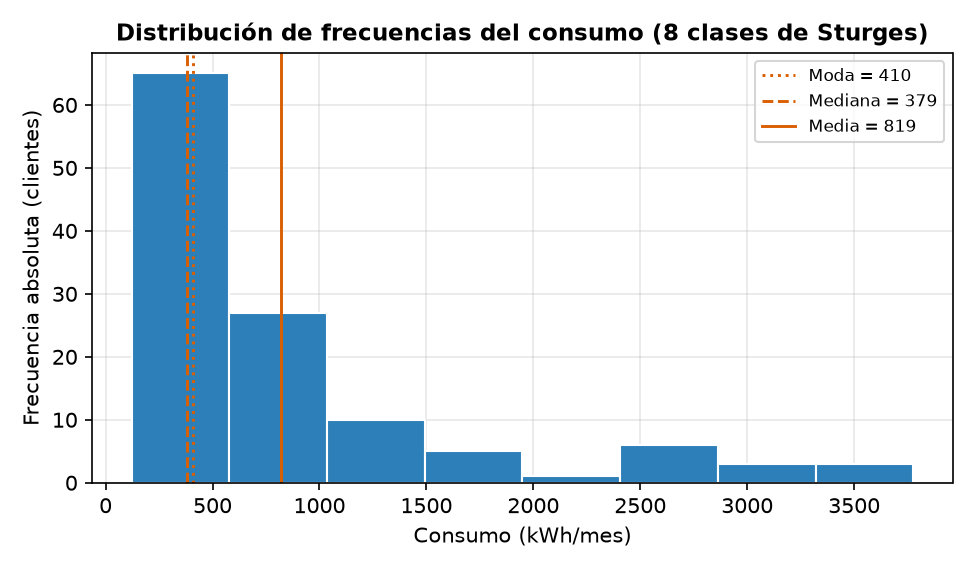
\includegraphics[width=\linewidth]{assets/images/figures/python/hist_sturges_central_tendency.png}
            \end{minipage}
            \hfill
            \begin{minipage}{0.49\textwidth}
                \centering
                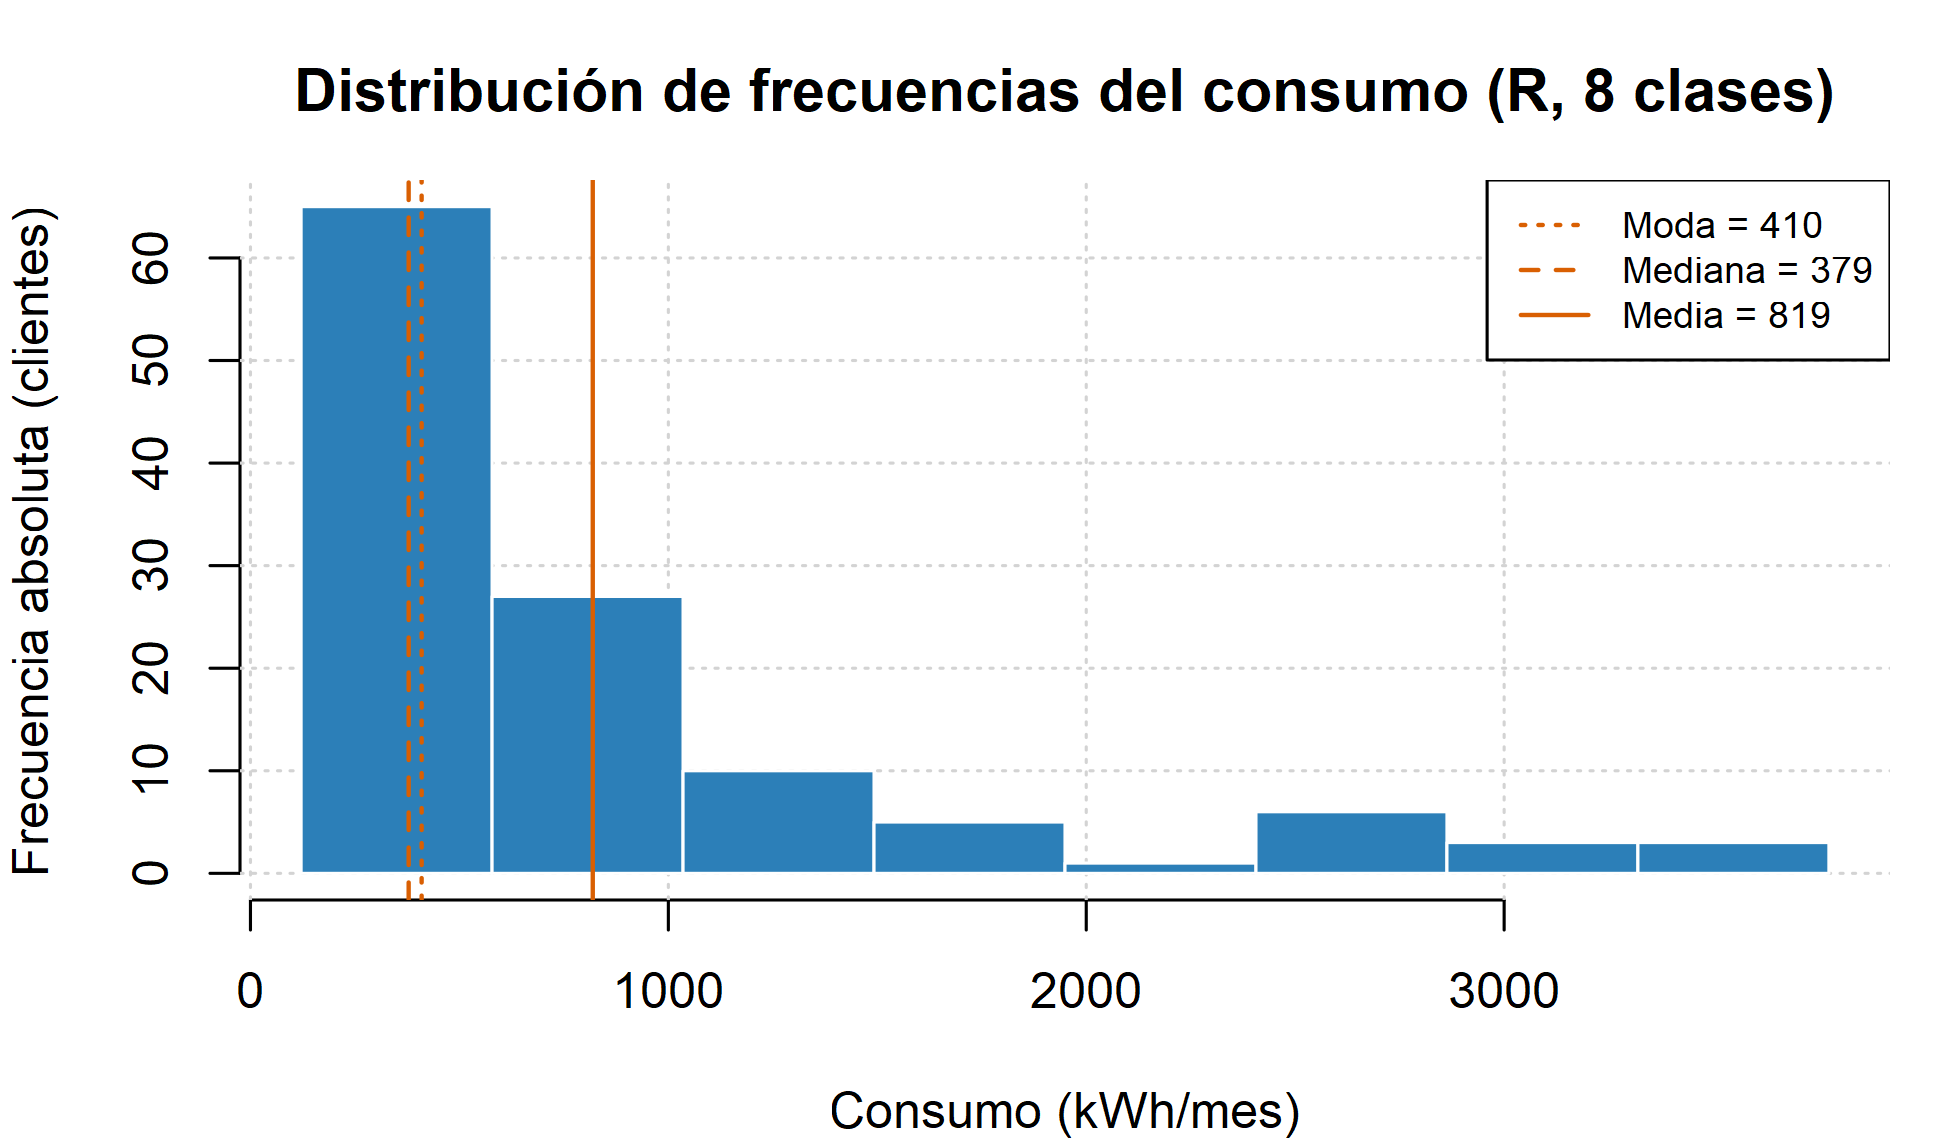
\includegraphics[width=\linewidth]{assets/images/figures/r/hist_sturges_central_tendency.png}
            \end{minipage}

            \vspace{4pt}

            \captionof{figure}{Distribución de frecuencias del consumo mensual con media,
            mediana y moda, en Matplotlib (izquierda) y su réplica en R (derecha)}
            \label{hist_sturges}
        \end{strip}

        La Figura \ref{polygon_ogive} presenta las otras dos representaciones de la
        misma tabla, el polígono de frecuencias y la ojiva, sobre la cual la horizontal
        del 50\% corta la curva en la mediana de aproximadamente 379 kWh. El polígono 
        comunica la misma información del histograma pero enfatiza la tendencia antes 
        que la magnitud de cada clase, mientras que la ojiva convierte la pregunta 
        ``cuántos clientes hay en esta clase'` en ``qué fracción del total queda por 
        debajo de este consumo'', permitiendo leer directamente sobre el eje cualquier 
        percentil, empezando por la mediana.

        \clearpage

        \begin{strip}
            \centering
            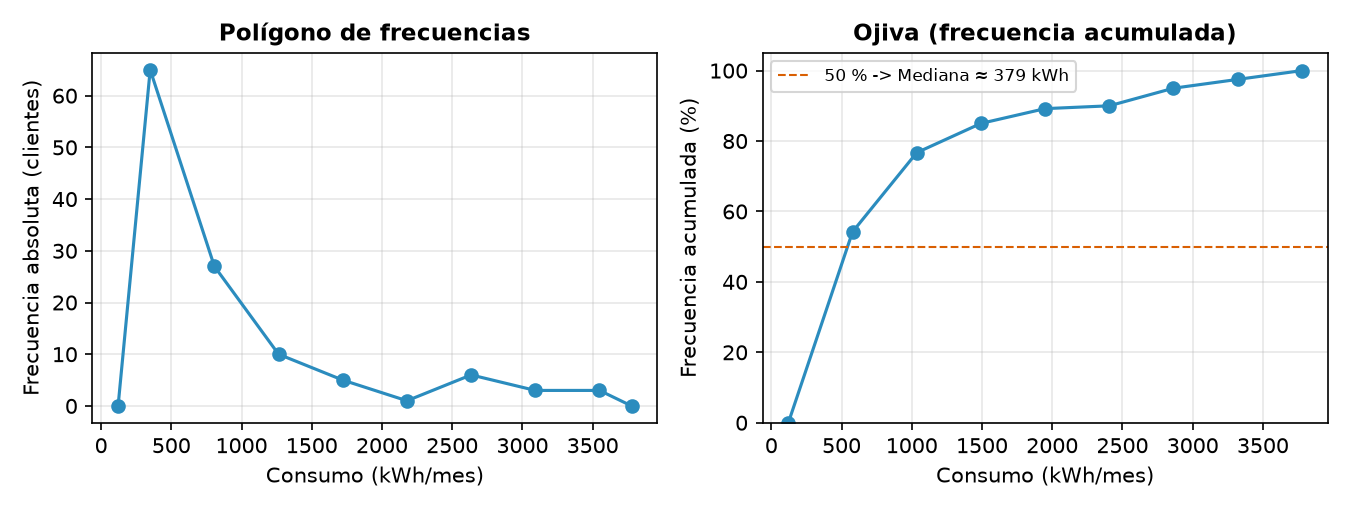
\includegraphics[width=0.86\linewidth]{assets/images/figures/python/freq_polygon_ogive.png}

            \vspace{6pt}

            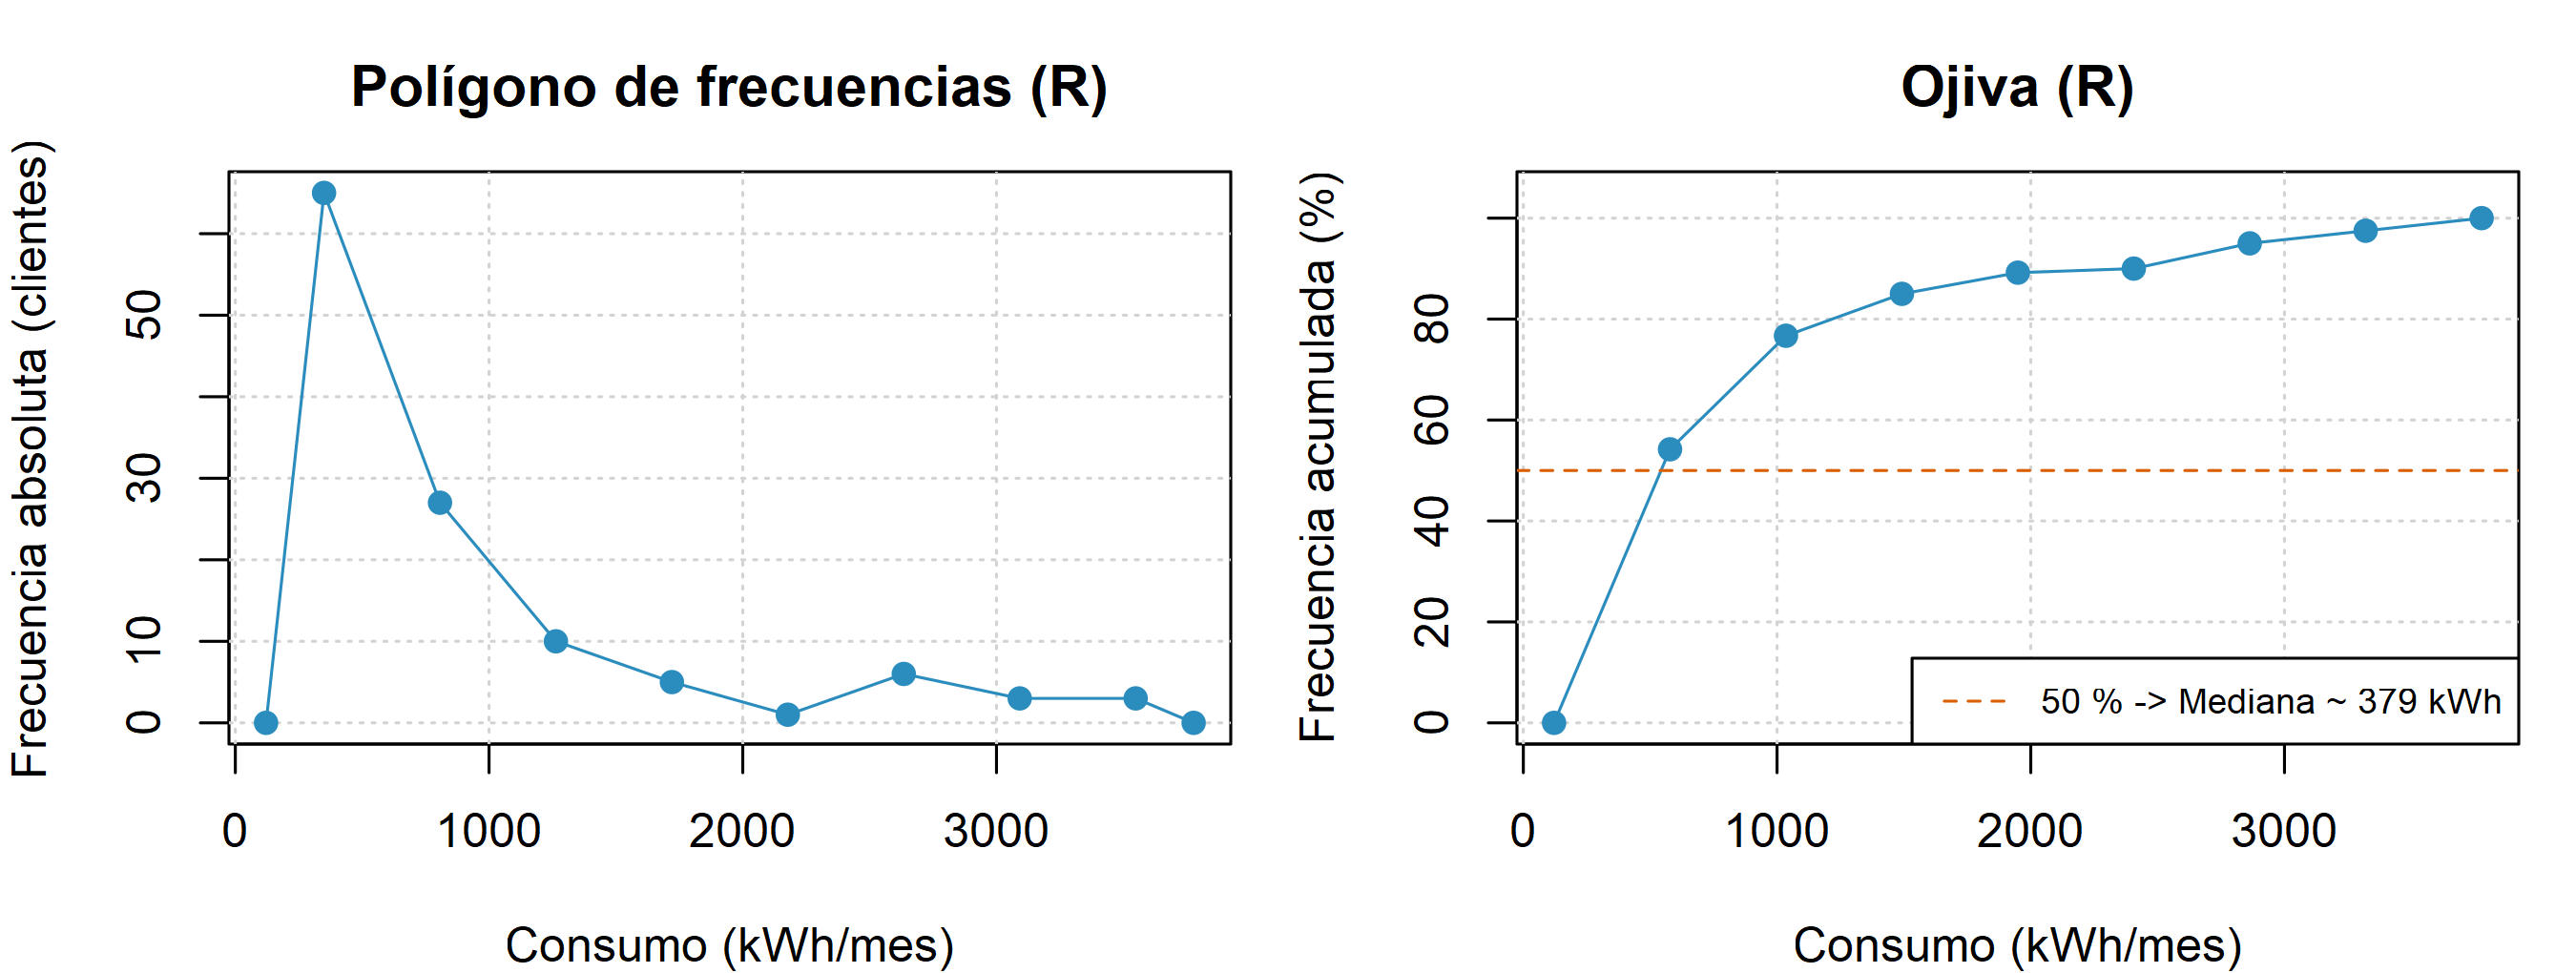
\includegraphics[width=0.86\linewidth]{assets/images/figures/r/freq_polygon_ogive.png}

            \vspace{4pt}

            \captionof{figure}{Polígono de frecuencias y ojiva del consumo mensual, en
            Matplotlib (arriba) y su réplica en R (abajo)}
            \label{polygon_ogive}
        \end{strip}

        La réplica en R exige un detalle de implementación que ilustra los principios de
        visualización, dado que la graficación base dibuja la cuadrícula encima de lo ya
        trazado, por lo que cada figura se construye en dos pasadas, la primera sin
        relleno para fijar los ejes y la escala, luego se inserta la cuadrícula y la
        segunda pasada dibuja los datos por encima, garantizando que la retícula quede
        siempre por detrás.

    \subsection{Medidas de tendencia central}
        La Tabla \ref{central_tendency} presenta la media, la mediana y la moda
        interpolada del consumo por sector y a nivel global. La moda de la variable
        nominal sector es Residencial, con 62 de los 120 clientes, equivalentes al
        52\%.

        \begin{table}[H]
            \centering
            \caption{Medidas de tendencia central del consumo mensual (kWh)}
            \begin{center}
                \begin{tabular}{|l|c|c|c|c|}
                    \hline
                    \textbf{Grupo} & $\mathbf{n}$ & \textbf{Media} & \textbf{Mediana} &
                    \textbf{Moda interp.} \\
                    \hline
                    Residencial & 62  & 248,3   & 240,6   & 232,7   \\
                    \hline
                    Comercial   & 40  & 878,1   & 866,6   & 787,8   \\
                    \hline
                    Industrial  & 18  & 2.654,0 & 2.666,8 & 1.849,3 \\
                    \hline
                    Global      & 120 & 819,1   & 378,6   & 409,6   \\
                    \hline
                \end{tabular}
                \label{central_tendency}
            \end{center}
        \end{table}

        El contraste entre los niveles de la tabla es el hallazgo central del análisis,
        puesto que dentro de cada sector la media y la mediana son casi iguales, con
        248,3 frente a 240,6 en Residencial, 878,1 frente a 866,6 en Comercial y
        2.654,0 frente a 2.666,8 en Industrial, lo que es una señal de distribuciones
        simétricas, y la moda interpolada industrial se aleja algo más por el tamaño
        reducido del grupo ($n = 18$), que hace inestable la clase modal.

        \vspace{10pt}

        A nivel global, en cambio, la media duplica con creces a la mediana, no porque
        existan datos atípicos sino porque el promedio mezcla tres poblaciones de
        escalas distintas. La Figura \ref{bar_sector} muestra la distribución de la
        variable nominal y compara la media con la mediana de cada sector, donde la casi
        igualdad de las parejas de barras hace visible la simetría interna de cada grupo.

        \vspace{10pt}

        El diagrama de barras es la representación propia de una variable nominal y por
        esa razón sus barras aparecen separadas, a diferencia del histograma que
        son contiguas porque el consumo es continuo, adicionalmente, las etiquetas de
        datos evitan que el lector deba estimar la altura contra el eje, aplicando el 
        principio de etiquetado completo \cite{few2012show}.

        \clearpage

        \begin{strip}
            \centering
            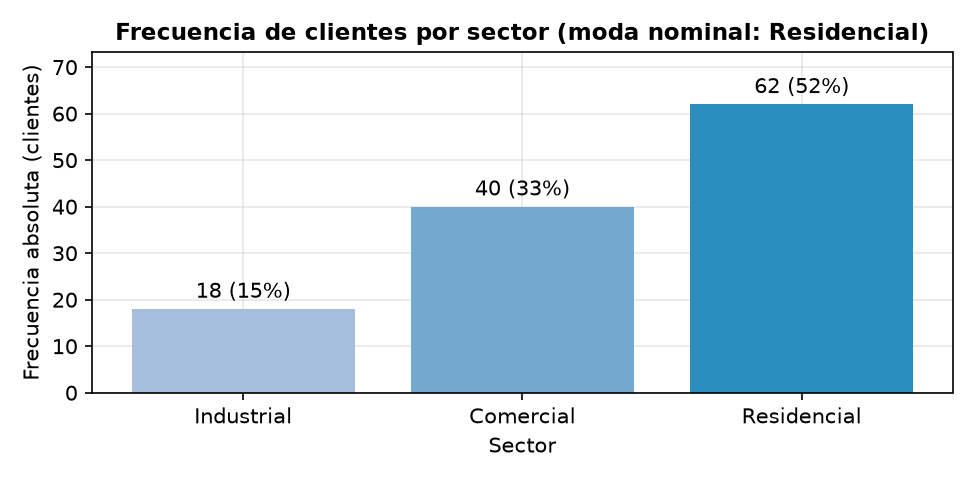
\includegraphics[width=0.45\linewidth]{assets/images/figures/python/bar_freq_by_sector.png}
            \hfill
            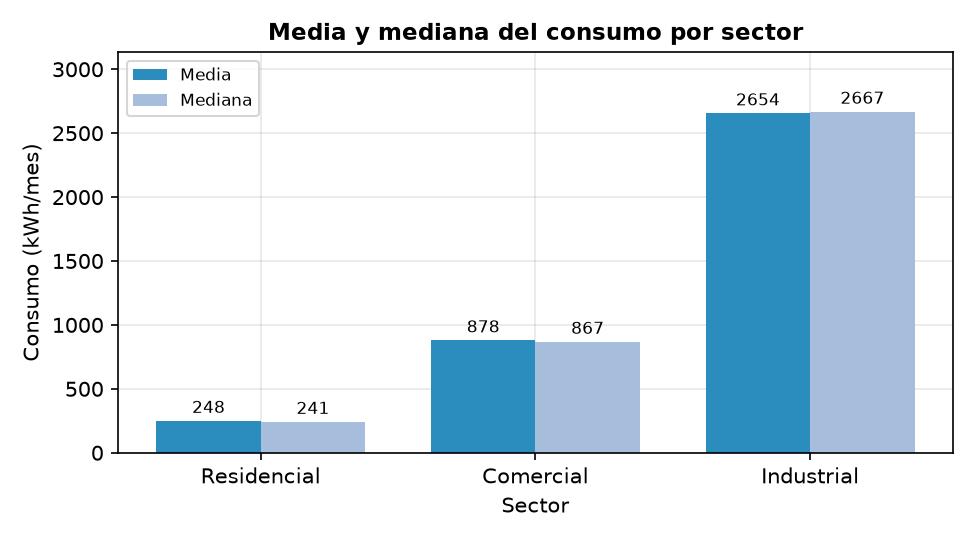
\includegraphics[width=0.45\linewidth]{assets/images/figures/python/bar_mean_median_by_sector.png}

            \vspace{6pt}

            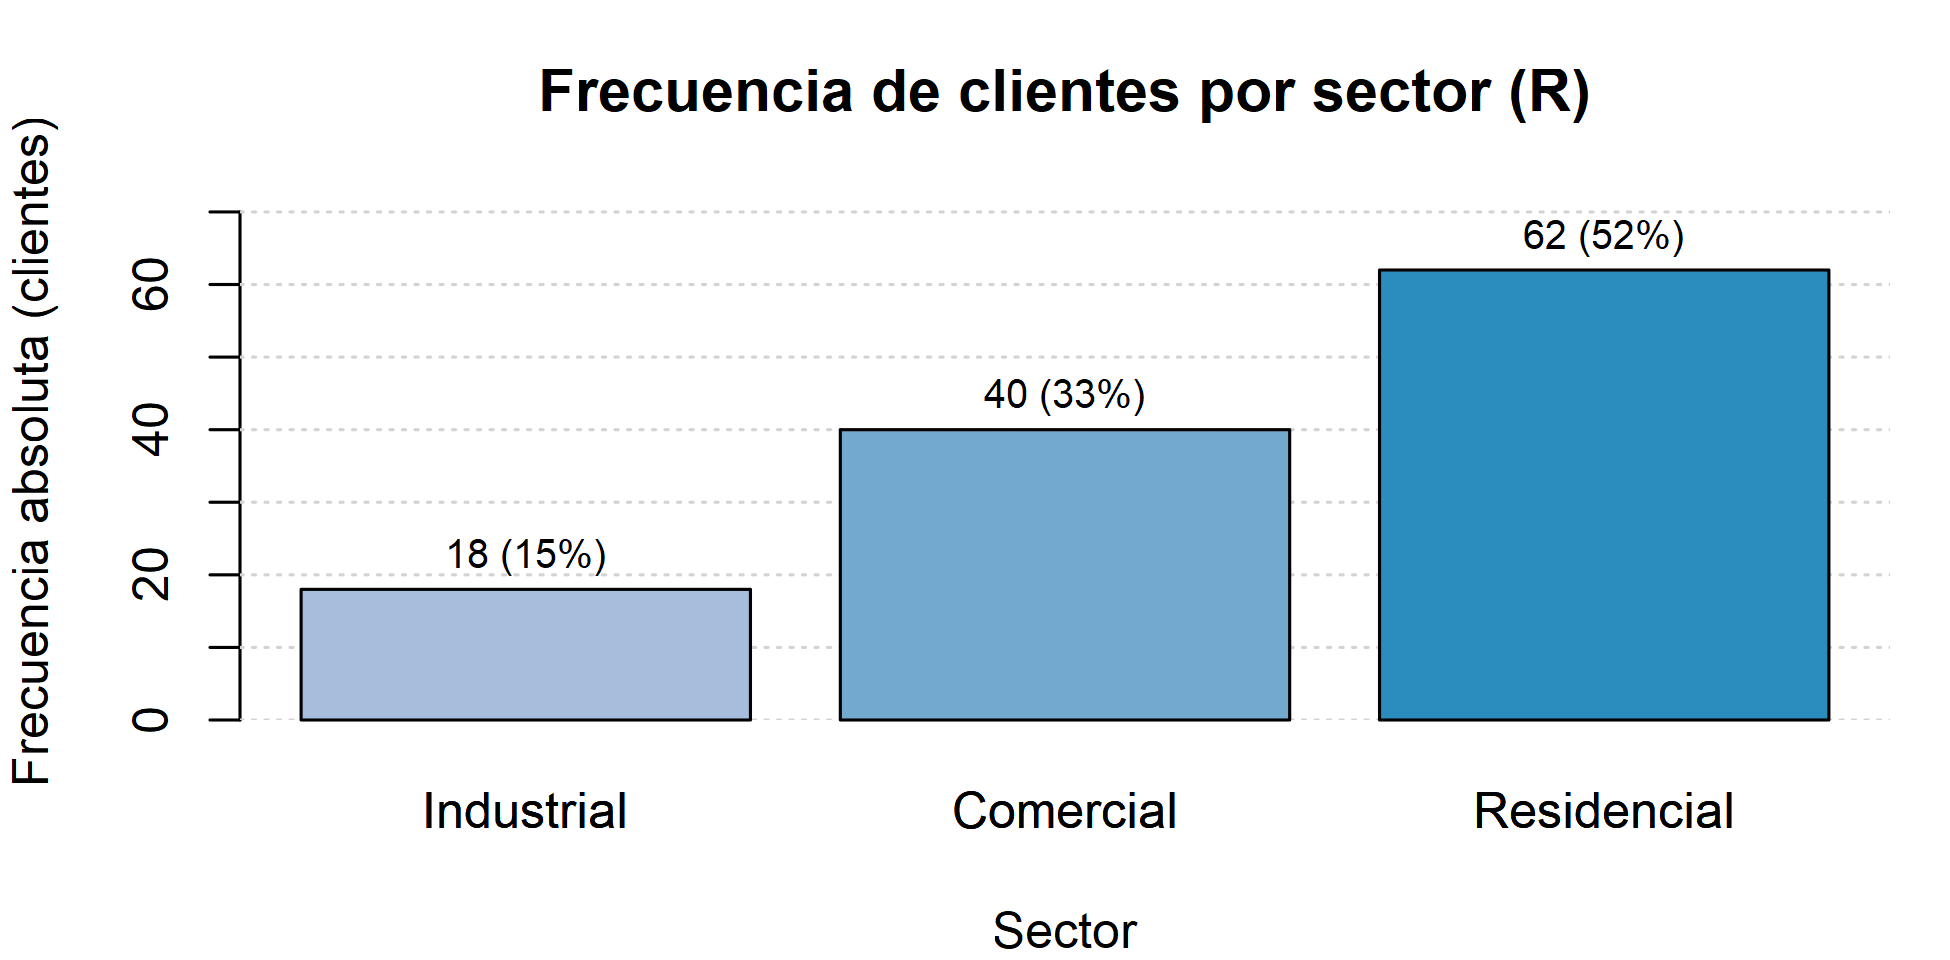
\includegraphics[width=0.45\linewidth]{assets/images/figures/r/bar_freq_by_sector.png}
            \hfill
            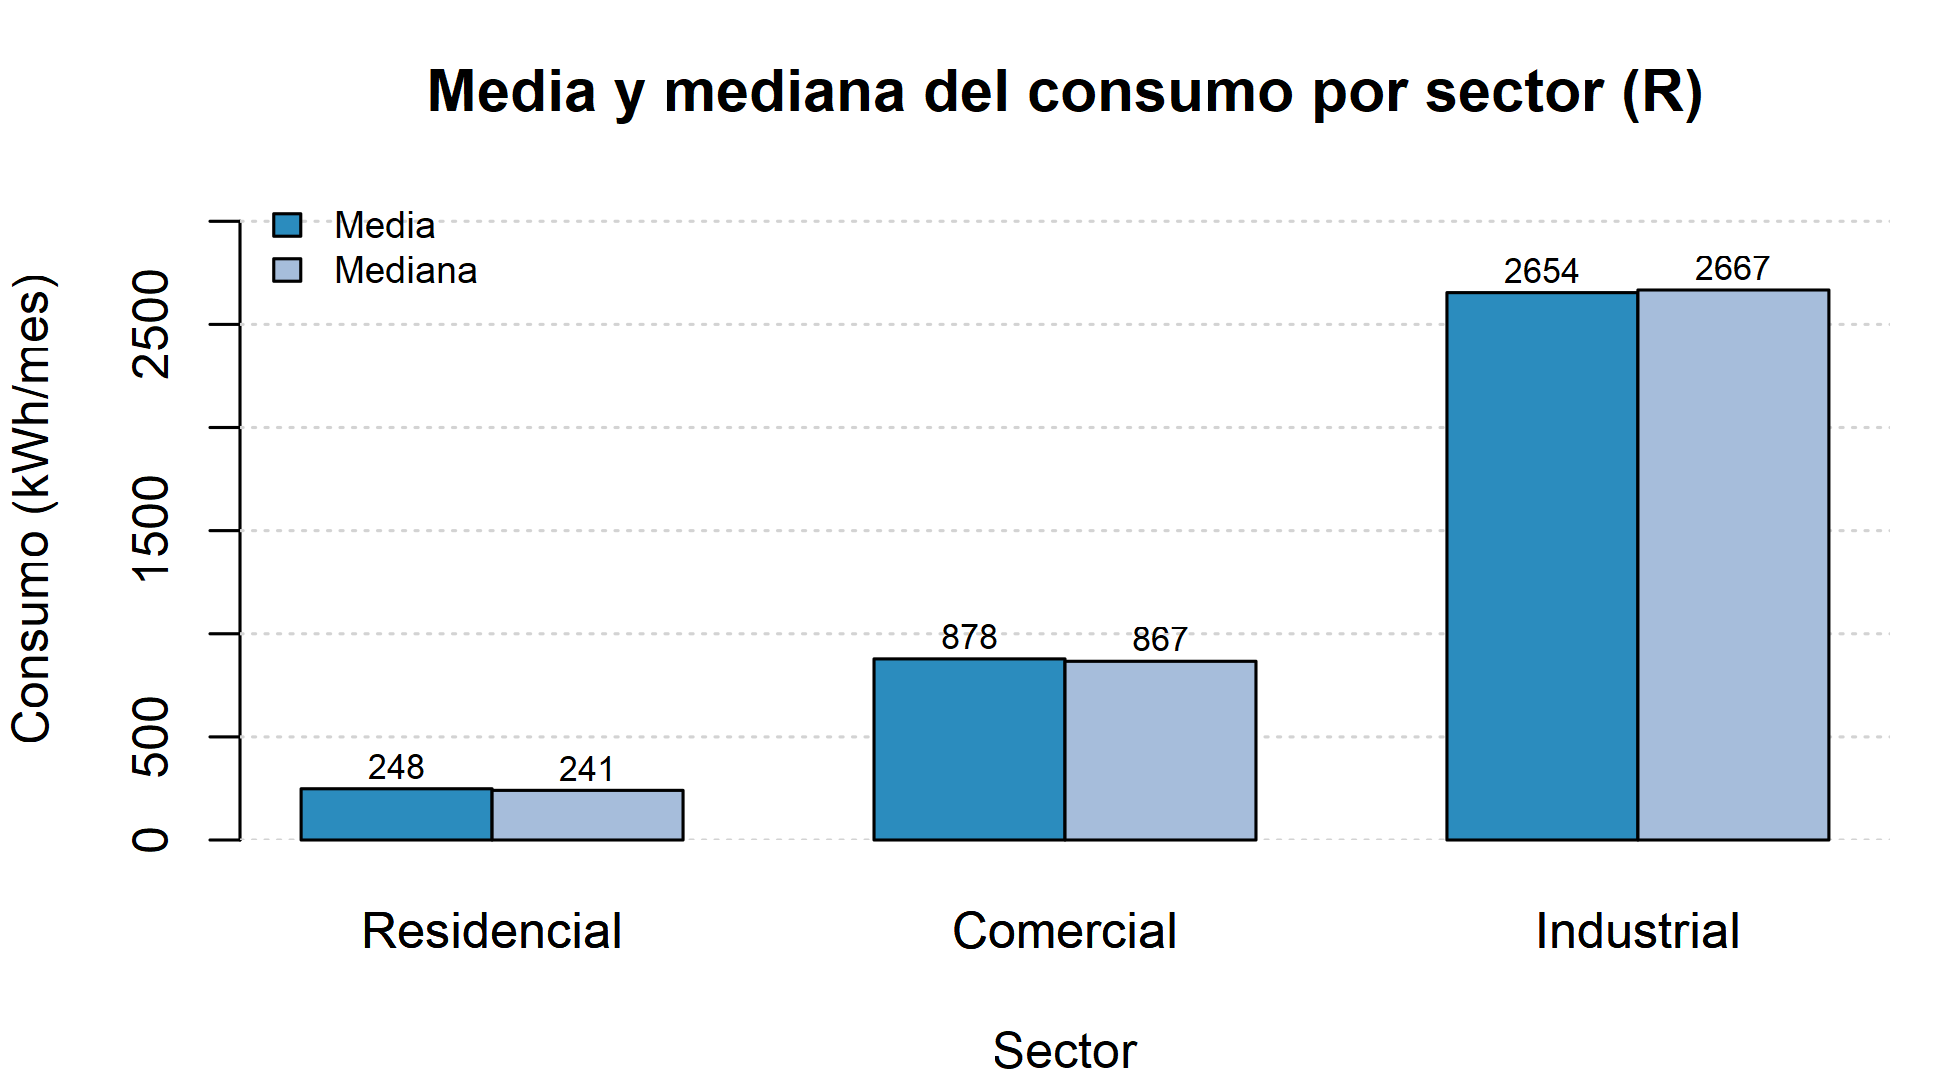
\includegraphics[width=0.45\linewidth]{assets/images/figures/r/bar_mean_median_by_sector.png}

            \vspace{4pt}

            \captionof{figure}{Frecuencia de clientes por sector con la moda nominal
            Residencial (izquierda) y comparación entre media y mediana por sector
            (derecha), en Matplotlib (arriba) y su réplica en R (abajo)}
            \label{bar_sector}
        \end{strip}

    \subsection{Medidas de dispersión}
        La Tabla \ref{dispersion} presenta las medidas de dispersión del consumo por
        sector y a nivel global, y la Figura \ref{boxplot_dispersion} las representa
        mediante el diagrama de caja con la media y la desviación estándar superpuestas.

        \begin{table}[H]
            \centering
            \caption{Medidas de dispersión del consumo mensual (kWh)}
            \begin{center}
                \begin{tabular}{|l|c|c|c|c|c|}
                    \hline
                    \textbf{Grupo} & \textbf{Rango} & \textbf{Varianza} &
                    $\mathbf{s}$ & \textbf{CV (\%)} & \textbf{IQR} \\
                    \hline
                    Residencial & 303,6   & 3.736,3   & 61,1  & 24,6  & 69,5    \\
                    \hline
                    Comercial   & 908,4   & 42.989,5  & 207,3 & 23,6  & 255,3   \\
                    \hline
                    Industrial  & 2.103,1 & 471.785,8 & 686,9 & 25,9  & 1.322,8 \\
                    \hline
                    Global      & 3.655,9 & 763.564,7 & 873,8 & 106,7 & 742,0   \\
                    \hline
                \end{tabular}
                \label{dispersion}
            \end{center}
        \end{table}

        Con el fin de representar las cifras obtenidas en su forma gráfica, la Figura
        \ref{boxplot_dispersion} traduce los valores de la Tabla \ref{dispersion} en el
        diagrama de caja, que resume en una sola imagen la posición de la mediana, la
        amplitud del rango intercuartílico y el alcance de los bigotes, con la media y la
        desviación estándar superpuestas en cada grupo, junto con su réplica en R, de
        esta manera, la brecha de escala entre sectores y la homogeneidad de su
        dispersión relativa, que en la tabla se leen número a número, se aprecian de un
        solo vistazo.

        \begin{figure}[H]
            \centering
            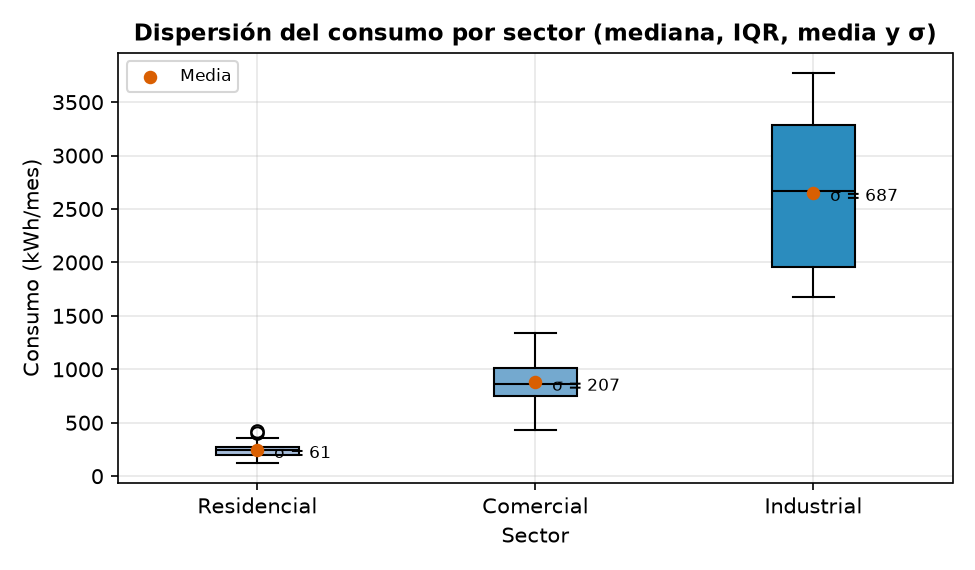
\includegraphics[width=1\linewidth]{assets/images/figures/python/boxplot_dispersion_by_sector.png}

            \vspace{4pt}

            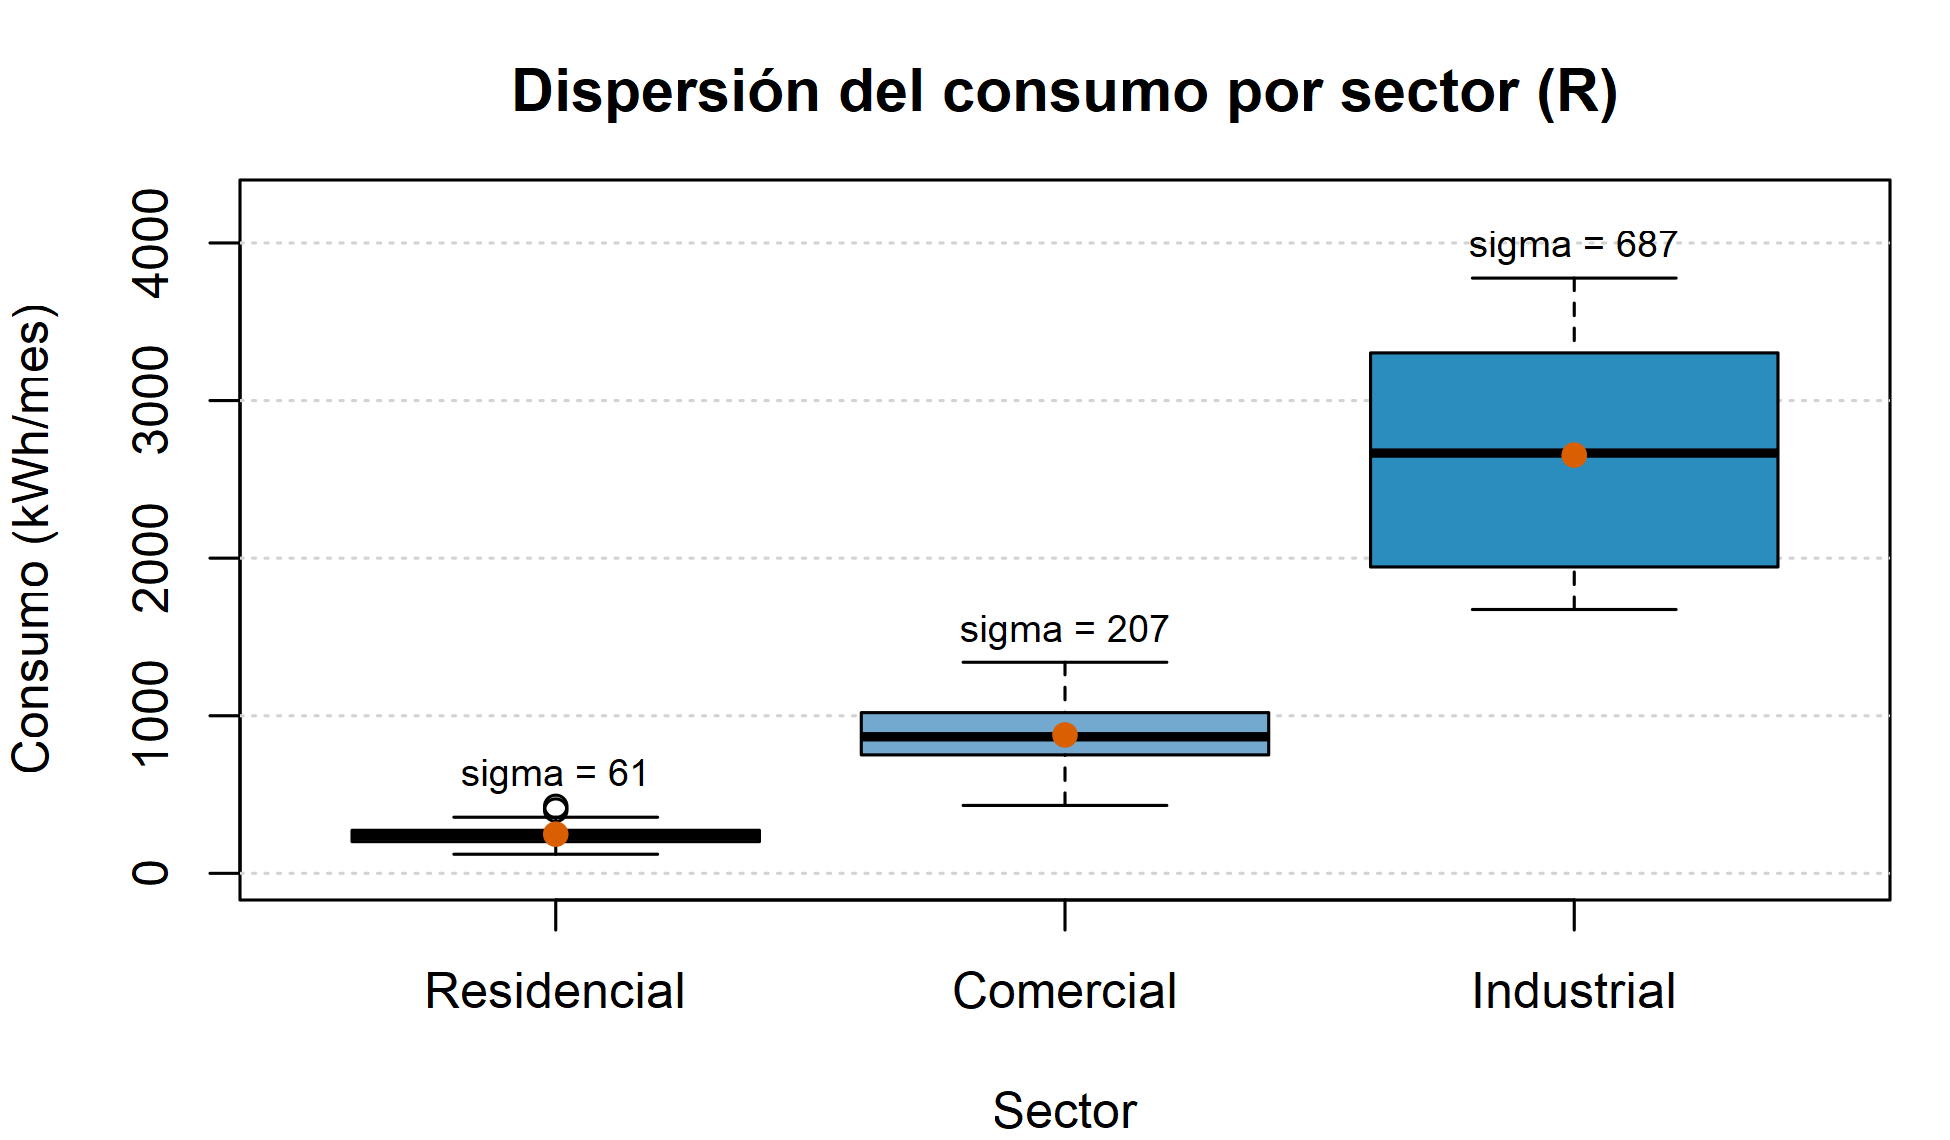
\includegraphics[width=1\linewidth]{assets/images/figures/r/boxplot_dispersion_by_sector.png}
            \caption{Dispersión del consumo por sector con mediana, IQR, media y
            $\sigma$, en Matplotlib (arriba) y su réplica en R (abajo)}
            \label{boxplot_dispersion}
        \end{figure}

        La lectura conjunta de la tabla y la figura arroja tres deducciones, la primera,
        que la dispersión absoluta crece con la escala del sector, pues la desviación
        estándar pasa de 61,1 kWh en Residencial a 686,9 kWh en Industrial y la varianza
        amplifica esa brecha en dos órdenes de magnitud, lo que en el diagrama de caja se
        aprecia como cajas y bigotes progresivamente más amplios, la segunda radica en
        que la dispersión relativa resulta homogénea, ya que el coeficiente de variación
        se mantiene entre 23,6\% y 25,9\% en los tres sectores, es decir, cada grupo
        es igualmente variable en proporción a su media y la tercera, que el CV global
        (106,7\%) cuadruplica al de cualquier sector, una explosión de variabilidad
        relativa que no proviene de la dispersión interna de los grupos sino de la
        distancia entre sus centros, lo que constituye la evidencia numérica de que el
        conjunto global es una mezcla de poblaciones, en plena coherencia con el vacío de
        la Tabla \ref{freq_table} y la separación sin traslape de las cajas en la Figura
        \ref{boxplot_dispersion}.

    \subsection{Verificación cruzada entre Python y R}
        El script de R recalculó de forma independiente la tabla de frecuencias completa,
        con las mismas ocho clases donde las medidas de tendencia central, incluida la
        moda interpolada por clase modal y las medidas de dispersión coinciden dígito a
        dígito con los resultados de Python, por ende, se puede concluir que la
        equivalencia entre \texttt{var()} y \texttt{sd()} de R y el parámetro
        \texttt{ddof=1} de pandas explica la coincidencia exacta de las varianzas
        muestrales. Las réplicas gráficas en sus paneles de R conservan además los
        principios de diseño, con la cuadrícula trazada en dos pasadas, confirmando que
        tanto los cálculos como su representación son independientes de la herramienta
        empleada.

